\subsection{Dataset and Event Selection}

\subsubsection{2016 \texorpdfstring{\pxPb}{p+Pb} Data}
The \pxPb\ data at \SNN~=~8.16~\TeV\ used for this analysis were delivered by the LHC to ATLAS in November and December of 2016. In \pxPb\ collisions at 8.16 \TeV\ the colliding beams have different energies per nucleon (6.5~\TeV\ protons colliding with $(Z/A)\times 6.5~\TeV\simeq 2.6~\TeV$ per nucleon in a lead nucleus), resulting in a collision system with \SNN~=~8.16~\TeV\ per nucleon pair. Under these conditions, the center-of-mass frame is shifted in rapidity, \RAP, by $\Delta\RAP=0.465$ in the direction of the proton beam. Data were collected in two different periods, characterized by opposite beam orientations. Due to technical issues with the ZDC instrumentation (see Section~\ref{sec:missing_zdc_mod}), only \textbf{Period B} was used for this measurement.

The runs in this period were characterized by a total integrated luminosity of 55.9~\NB. Beam 1 consisted of protons and Beam 2 of Pb ions. The protons traveled toward negative rapidities in the ``A$\rightarrow$C'' direction, corresponding to clockwise motion in the accelerator according to ATLAS conventions. This is denoted as the \pxPb\ configuration. All data sets used in this analysis, listed in Table~\ref{tab:datasets}, were processed using \textsc{ATHENA}~Release~21.

\begin{table}[ht]
    \centering
    \begin{tabular}{ | c | c |}
        \hline
        \rule{0pt}{2.25ex}
        \textbf{2016 \SNN\ = 8.16 \TeV\ Data Samples}  & \textcolor{black}{ \textbf{Luminosity [nb$^{-1}$] } } \\
        \hline
        \hline
        data16\_hip8TeV.00313063.physics\_Main.merge.AOD.r11416\_p3868 & 0.021 \\
        \hline
        data16\_hip8TeV.00313067.physics\_Main.merge.AOD.r11416\_p3868 & 0.486 \\
        \hline
        data16\_hip8TeV.00313100.physics\_Main.merge.AOD.r11416\_p3868 & 8.787 \\
        \hline
        data16\_hip8TeV.00313107.physics\_Main.merge.AOD.r11416\_p3868 & 11.053 \\
        \hline
        data16\_hip8TeV.00313136.physics\_Main.merge.AOD.r11416\_p3868 & 9.602 \\
        \hline
        data16\_hip8TeV.00313187.physics\_Main.merge.AOD.r11416\_p3868 & 3.030 \\
        \hline
        data16\_hip8TeV.00313259.physics\_Main.merge.AOD.r11416\_p3868 & 4.659 \\
        \hline
        data16\_hip8TeV.00313285.physics\_Main.merge.AOD.r11416\_p3868 & 4.272 \\
        \hline
        data16\_hip8TeV.00313295.physics\_Main.merge.AOD.r11416\_p3868 & 9.923 \\
        \hline
        data16\_hip8TeV.00313333.physics\_Main.merge.AOD.r11416\_p3868 & 3.791 \\
        \hline
        data16\_hip8TeV.00313435.physics\_Main.merge.AOD.r11416\_p3868 & 0.301 \\
        \hline
        \hline
    \end{tabular}
    \caption{\textcolor{black}{Data samples from \SNN\,= 8.16 \TeV\,\pxPb\,collisions collected during the 2016 Heavy Ion Run. The luminosity collected for each run is reported. All the data were processed using \textsc{ATHENA}~Release~21.}}
    \label{tab:datasets}
\end{table}

\subsubsection{Trigger Configuration}

\subsubsection{Monte Carlo Samples}

In order to evaluate the performance of jet reconstruction and the jet response within ATLAS, dijet Monte Carlo samples generated using \pythia~\cite{Bierlich:2022pfr} with the A14 tune and the NNPDF23LO PDFs~\cite{Ball:2012cx} were produced. Dijet events are filtered using the JZ$*$R04 filters, which select events containing an \antikt\~R~=~0.4 jet in specific truth \PT{} ranges, refered to using the prefix `JZ' and an integer ranging from 1--5 in this analysis.
The detector response was simulated using the full ATLAS detector simulation based on the Geant4 toolkit~\cite{Agostinelli:2002hh}. For \pxPb\ collisions, Pythia8 truth events are overlaid with real minimum-bias \pxPb\ data. For each event, the Pythia generation and subsequent simulations were run with conditions matching the collected data, allowing for the simulation to account for underlying event effects in the jet reconstruction. Please note that, in this MC sample, the event activity is originated mainly from the overlay contribution, and therefore has no truth associated.





Events are required to satisfy detector and data-quality requirements, contain
at least one reconstructed primary vertex, and contain two reconstructed jets.
Fully efficient central and forward single-jet triggers with different
transverse-momentum thresholds provide coverage over the analysis phase space.
Jets are reconstructed from calorimeter towers with the anti-$k_t$ algorithm,
using E-scheme recombination and radius parameter $R=0.4$. The leading and
subleading jets are required to satisfy $p_{\mathrm{T},1}>40~\mathrm{GeV}$ and
$p_{\mathrm{T},2}>30~\mathrm{GeV}$, respectively, with
$-2.8<\eta_{1,2}<4.5$. The asymmetric pseudorapidity selection prevents the
jets from biasing the Pb-going FCal estimator.

Events with either selected jet near the disabled hadronic endcap calorimeter
sector are removed. The excluded region is enlarged by 0.4 in both
pseudorapidity and azimuth, and the corresponding efficiency is included in
the detector correction. The analysis considers the 0--90\% event-activity
interval, suppressing ultra-peripheral-collision contamination. In-time pileup
is rejected by requiring that no non-primary vertex has more than six associated
tracks. A ZDC pre-sample requirement rejects events with elevated baselines
from preceding interactions, thereby removing residual out-of-time pileup that
can distort the FCal energy measurement.

Detector effects are evaluated with \textsc{Pythia} dijet events overlaid with
minimum-bias $p$+Pb data during detector simulation. The simulated FCal
distribution is reweighted at the event level to match that of the dijet data.

\subsubsection{Missing ZDC Module on Side C}
\label{sec:missing_zdc_mod}
During the 2016 \pxPb\ run, the ZDC side C module 0 (EM) was removed and replaced with the Arm2 calorimeter of the LHCf experiment~\cite{Adriani:2135330}. Figure~\ref{fig:lhcf_v_zdc_acceptance} displays the transverse acceptance of both the ATLAS ZDC and LHCf.  The ATLAS ZDC EM Module is the first of 4 sequential calorimeter modules (counting from the perspective of looking at the ZDCs from the ATLAS interaction point); therefore, the LHCf calorimeter would see forward neutral products before they reach the side C ZDC.  The LHCf detector was put in place to measure the forward neutral products of the proton going side in the \pxPb\ orientation; however, in the \Pbxp\ orientation the LHCf detector was retracted into the ``garage'' position to avoid radiation damage~\cite{Adriani:2135330}.  The ``garage'' position indicates an upwards vertical shift of 112 mm from the nominal position shown in Figure~\ref{fig:lhcf_v_zdc_acceptance}.  This shift places the full LHCf Arm2 calorimeter outside of the full acceptance of the ATLAS ZDC.  Still, the side C ZDC suffers from only having roughly 75~\% of the material budget of side A. This effectively reduces the interaction length of the side C ZDC from 4.6 to 3.4, which in turn reduces the neutrons expected to shower in the ZDC from 99\% to 96.6\%. For this reason, in this analysis only Period B (\pxPb), is used to obtain the final results.

\begin{figure}[p]
    \centering
    \begin{subfigure}[c]{0.45\linewidth}
        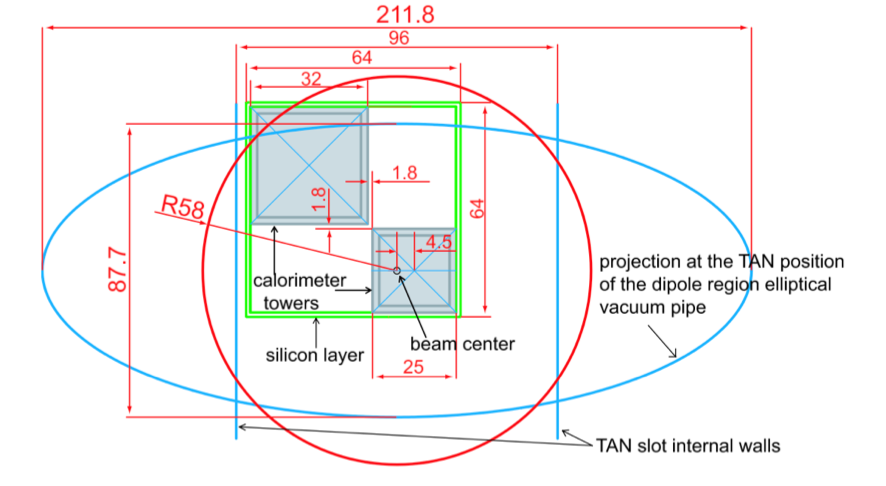
\includegraphics[
            width=1\linewidth,
            alt={Transverse acceptance of the LHCf Arm2 calorimeter viewed from the ATLAS interaction point.}
        ]{chapters/geometry_estimators_pPb/figures/dataset_and_event_selection/lhcfAcceptence.png}
    \end{subfigure}
    \begin{subfigure}[c]{0.45\linewidth}
        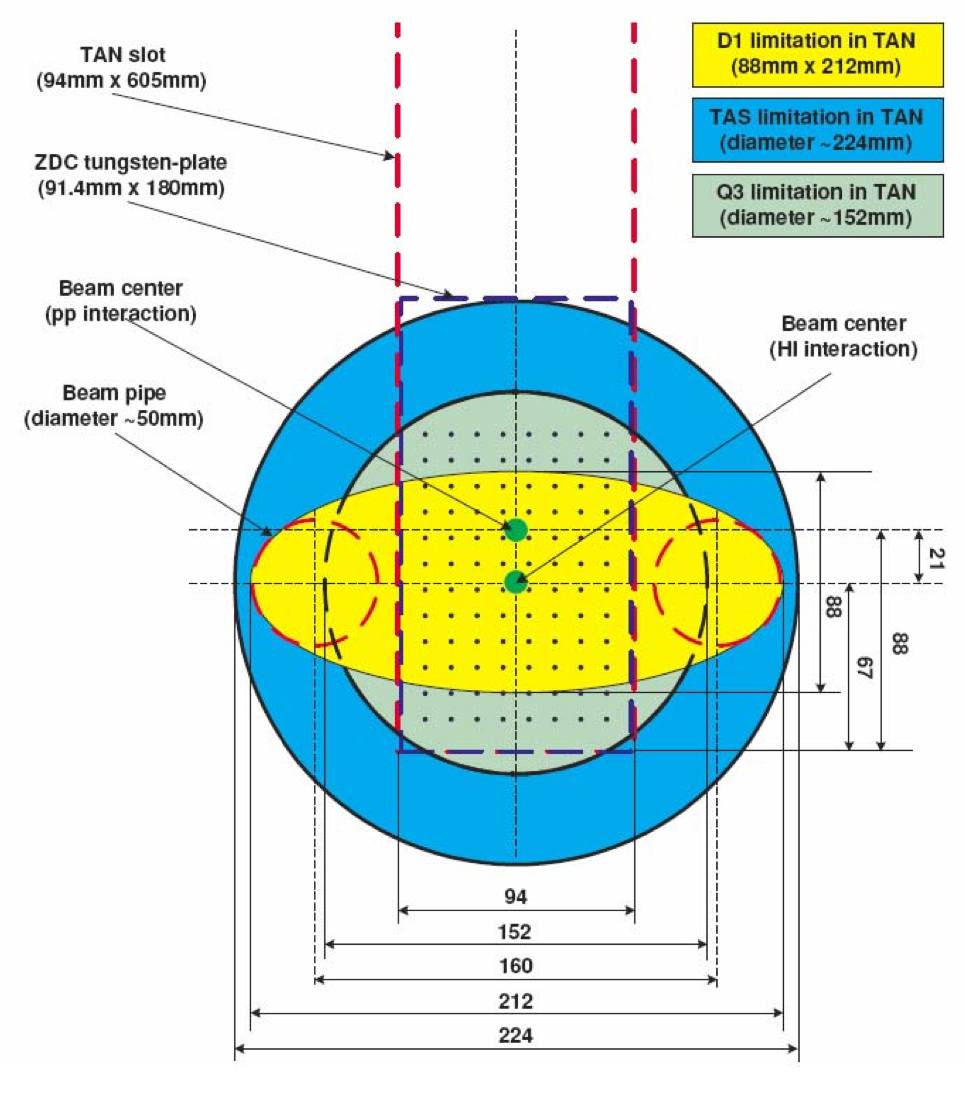
\includegraphics[
            width=1\linewidth,
            alt={Transverse acceptance of the ATLAS ZDC viewed from the ATLAS interaction point.}
        ]{chapters/geometry_estimators_pPb/figures/dataset_and_event_selection/zdcAcceptence.png}
    \end{subfigure}
    \caption{Detector Geometry for LHCf Arm2~\cite{Cekmecelioglu:2867369} (left) and the ATLAS ZDC~\cite{Jenni:1009649} (right). View is from the perspective of the ATLAS interaction point. In both figures the distances are given in mm.  The blue oval in the left image corresponds to the boundary of the yellow oval in the right image.  The active area of LHCf is represented by the filled blue squares.  The active area of the ZDC is given by the area bounded by the purple dashed line.}
    \label{fig:lhcf_v_zdc_acceptance}
\end{figure}

In the \pxPb\ orientation, the LHCf was in running position in runs 313063 and 313435, while for all other runs it was in ``garage'' position. Due to the asymmetric design of the LHCf module in the transverse plane, the effect on the acceptance of the ZDC in the proton-going direction during these runs is nontrivial. Any measurement in this thesis using the proton-going ZDC excludes these runs.
